%\documentclass[notes]{beamer}       % print frame + notes
%\documentclass[notes=only]{beamer}   % only notes
\documentclass{beamer}              % only frames
  \usepackage[english]{babel}
\usepackage[round]{natbib}
%\documentclass[hyperref={pdfpagelabels=false}]{beamer}
\usepackage{lmodern}
\usepackage{marvosym} % \MVRIGHTarrow

\usepackage{amsmath}  
\usepackage{multirow,graphicx,array}
\usepackage{multicol}
\usepackage{hhline}
\usepackage{xcolor}
\usepackage{colortbl}
\usepackage{threeparttable,booktabs}
\usepackage{chngcntr}
\usepackage{dcolumn}
\usepackage{caption}
\usepackage{fixltx2e}
\usepackage{rotating}
\usepackage{amssymb}
 \usepackage{setspace}
\usepackage{changepage}
\usetheme{Singapore}
\useoutertheme{miniframes}
\AtBeginSection[]{\subsection{}}


\newcommand{\RowColor}{\rowcolor{gray} \cellcolor{white}}
\newcommand{\RowColorY}{\rowcolor{yellow} \cellcolor{white}}



\newcommand{\RN}[1]{%
  \textup{\uppercase\expandafter{\romannumeral#1}}%
}

\newcommand\Wider[2][3em]{%
\makebox[\linewidth][c]{%
  \begin{minipage}{\dimexpr\textwidth+#1\relax}
  \raggedright#2
  \end{minipage}%
  }%
}




\title{Effects of Weather on Maize Yield in Kenya}  
\author{Monika Novackova \\[2mm] \footnotesize supervised by: \textcolor{darkblue}{Pedram Rowhani, Martin Todd and Annemie Maertens}} 

\date{January 2019} 
\institute{University of Sussex}

\setbeamercolor{block title}{bg=purple!30,fg=black}





\begin{document}


\definecolor{LightCyan}{rgb}{0.88,1,1}
\definecolor{BeigeNadine}{rgb}{1,0.94,0.86}
\definecolor{DarkGreen}{rgb}{0.1803922,0.545098,0.3411765}
\definecolor{BeigeNadine}{rgb}{1,0.94,0.86}
\definecolor{PaleGreen}{rgb}{ 0.5960784,0.9843137, 0.5960784}
\definecolor{darkblue}{rgb}{0.0, 0.0, 0.55}
\definecolor{bored}{rgb}{0.8, 0.0, 0.0}
\definecolor{babypink}{rgb}{0.96, 0.76, 0.76}

 \newcolumntype{d}{D{.}{.}{-1}}
 \newcolumntype{e}{D{+}{\,\pm\,}{6,2}}




\maketitle


\normalsize

\begin{frame}
\frametitle{Outline}
\tableofcontents
\end{frame} 

\note{A}



\section{Introduction}


%oooooooooooooooooooooooooooooooooooooooooooooooooooooooooooooooooooooooooooooooooooooooooooooooooooooooooooooooooooooooooooooooooooooooooooooooooooooooooooooooooooooooooooooooooooo
%oooooooooooooooooooooooooooooooooooooooooooooooooooooooooooooooooooooooooooooooooooooooooooooooooooooooooooooooooooooooooooooooooooooooooooooooooooooooooooooooooooooooooooooooooooo

\begin{frame}\label{Introduction}
\frametitle{Introduction} 
 \begin{itemize}
\item SSRP project, related to ForPAc project
\item Extreme weather $\rightarrow$ disasters \textcolor{red}{(maybe name some years of drought in Kenya??)}

\begin{itemize}
\item Early warning systems have been developed
\end{itemize}
\item Goals: Improve early warning systems in Kenya
\item Shifting the disaster management from reactive to protective
\end{itemize} 

\begin{itemize}
\item Two predominant rainfall regimes in Kenya:

\begin{enumerate}
\item Arid and semi-arid (ASAL): bi-modal
	\begin{itemize}
	\item Short rains: March to May
	\item Long rains: October to December
	\end{itemize}
\item non-ASAL: uni-modal
	\begin{itemize}
	\item March to August
	\end{itemize}

\end{enumerate}
\item \textcolor{red}{Perhaps a map of ASAL and non-ASAL}

\end{itemize}
\end{frame}

\note{Climate change has been increasing amplitudes and frequency of extreme weather events\\ Not every hazard turns into disaster
r
b}

%oooooooooooooooooooooooooooooooooooooooooooooooooooooooooooooooooooooooooooooooooooooooooooooooooooooooooooooooooooooooooooooooooooooooooooooooooooooooooooooooooooooooooooooooooooo
%oooooooooooooooooooooooooooooooooooooooooooooooooooooooooooooooooooooooooooooooooooooooooooooooooooooooooooooooooooooooooooooooooooooooooooooooooooooooooooooooooooooooooooooooooooo

\begin{frame}\label{Approaches00}
\frametitle{Approach} 


\begin{itemize}
\item Various approaches considered including:

\begin{itemize}
\item Relating NDMA Early warning phase classification to weather
\item Relating markets and food prices to weather
\item Relating maize yields to weather to weather
\item Computable general equilibrium (CGE) models
\end{itemize}
\end{itemize}
\end{frame}

\note{
Relating NDMA Early warning classification to weather also various precip and weather indexes
r
b}
%oooooooooooooooooooooooooooooooooooooooooooooooooooooooooooooooooooooooooooooooooooooooooooooooooooooooooooooooooooooooooooooooooooooooooooooooooooooooooooooooooooooooooooooooooooo
%oooooooooooooooooooooooooooooooooooooooooooooooooooooooooooooooooooooooooooooooooooooooooooooooooooooooooooooooooooooooooooooooooooooooooooooooooooooooooooooooooooooooooooooooooooo

\begin{frame}\label{Approaches01}
       \hspace{-0.8cm}  \textbf{NDMA Early Warning Phase\\ \hspace{-0.8cm} Classification}
        
\vspace{-0.9cm}
     \begin{figure}
      \begin{columns}
        \column{.4\linewidth}
       
  \caption*{\textcolor{DarkGreen}{\textbf{\underline{\small{Example: Kitui county}}}}\\
   
 \vspace{0.25cm}\hspace{-0.25cm} \textbf{\textit{\textcolor{blue}{Normal $\rightarrow$ Alert $\rightarrow$  Alarm}}} \\
   \vspace{0.4cm}  
 \hspace{-0.25cm}  $\bullet$ \small{Bulletins for ASAL counties} \\
   \hspace{-0.25cm}  $\bullet$ \small{Online since 2013} \\
     \vspace{0.1cm}  
  \hspace{0.15cm}    \footnotesize{$\bullet$ But in pdf format} \\ 
    \vspace{0.1cm}  
\hspace{-0.25cm}   \small{$\bullet$ For county and month}
 
 }
        \column{.6\linewidth}

    \vspace{-0.16cm}   \hspace{-0.1cm}   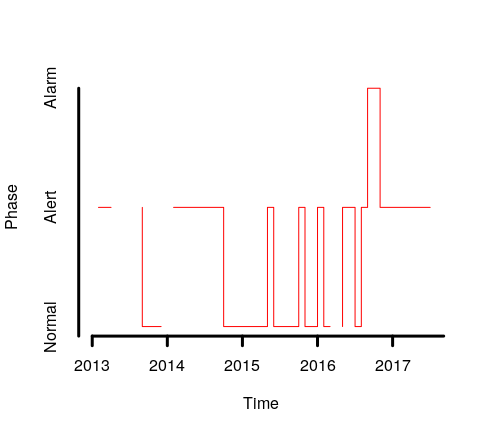
\includegraphics[width = 0.9\textwidth]{PhaseNA.png}  %565*238
 \vspace{-0.3cm}  
      \end{columns}
    \end{figure}
   
\vspace{-1.3cm}
    \begin{figure}
      \begin{columns}
        \column{.5\linewidth }
  \vspace{-1.8cm}        
        \column{.5\linewidth}
  \hspace{-2.6cm}  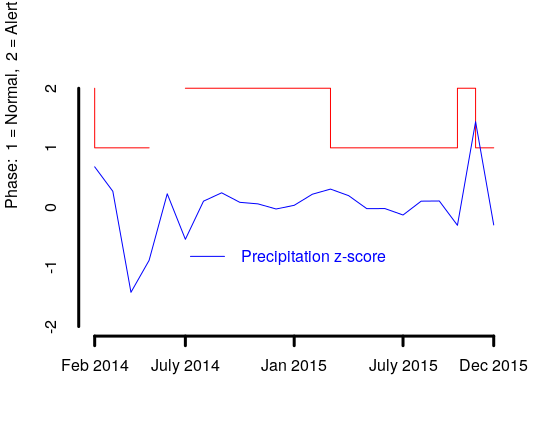
\includegraphics[width = 1.2\textwidth]{PrecNA.png}  %565*238
      \end{columns}
    \end{figure}

\end{frame}


\note{This is an example of one of the approaches that we eventually abandoned\\
b}




%oooooooooooooooooooooooooooooooooooooooooooooooooooooooooooooooooooooooooooooooooooooooooooooooooooooooooooooooooooooooooooooooooooooooooooooooooooooooooooooooooooooooooooooooooooo
%oooooooooooooooooooooooooooooooooooooooooooooooooooooooooooooooooooooooooooooooooooooooooooooooooooooooooooooooooooooooooooooooooooooooooooooooooooooooooooooooooooooooooooooooooooo

\begin{frame}\label{Approach}
\frametitle{Approach} 

\begin{itemize}
\item Narrowing the research question:
\begin{itemize}
\item Relationship of maize yield and weather in Kenya
\begin{itemize}
\item What is it about weather that causes drought related disasters?
\item Which particular characteristics of weather are the most 'responsible' for drought related disasters?
\end{itemize}
\end{itemize}
\end{itemize}

Sample:
\begin{itemize}
\item Panel of 47 counties of Kenya, $1981-2017$
\end{itemize}

\end{frame}

\note{After various problems with data (prices - not for every county, NDMA phases - not much of an objective criterion, probably political, various VCI values)
\\ so the decision about the approach was partially driven by data (un)availability}

%oooooooooooooooooooooooooooooooooooooooooooooooooooooooooooooooooooooooooooooooooooooooooooooooooooooooooooooooooooooooooooooooooooooooooooooooooooooooooooooooooooooooooooooooooooo
%oooooooooooooooooooooooooooooooooooooooooooooooooooooooooooooooooooooooooooooooooooooooooooooooooooooooooooooooooooooooooooooooooooooooooooooooooooooooooooooooooooooooooooooooooooo
\section{Data}
\begin{frame}\label{Data}
\frametitle{Data} 

\begin{itemize}
\item Maize yields
\begin{itemize}
\item source: Famine Early Warning Systems Network (FEWS NET)
\item County level, yearly, tonnes per hectare
\end{itemize}
\item Weather:
\begin{itemize}
\item Daily, $0.25^{\circ}$ resolution gridded data
\item Precipitation
	\begin{itemize}
	\item source: Climate Hazards Group InfraRed Precipitation with Station data (CHIRPS)
	\end{itemize}
\item Temperature
	\begin{itemize}
	\item source: Berkeley Earth
	\end{itemize}
	\item[$\blacksquare$] \textcolor{darkblue}{Aggregation needed to conform with the yield data}
	\end{itemize}

\end{itemize}

\begin{columns}
\footnotesize
	\begin{column}{0.4\textwidth}

	\end{column}
	\begin{column}{0.15\textwidth}
  		$0.25^{\circ}$ grid \\ daily
	\end{column}
	\begin{column}{0.05\textwidth}
  			$\rightarrow$ \\ $\rightarrow$
	\end{column}
	\begin{column}{0.25\textwidth} 
   		county level \\  yearly 
   	\end{column}
   		\begin{column}{0.4\textwidth} 
   		\end{column}
\end{columns}
\textcolor{red}{add how averaged over seasons ASAL and non ASAL}


\end{frame}

\note{After various problems with data (prices - not for every county, NDMA phases - not much of an objective criterion, probably political, various VCI values)
\\ so the decision about the approach was partially driven by data (un)availability \\ precip in mm, not sure if to put it into presentation as I would have to talk about units of temperature, mostly Kelvin but sometimes Celsius}

%oooooooooooooooooooooooooooooooooooooooooooooooooooooooooooooooooooooooooooooooooooooooooooooooooooooooooooooooooooooooooooooooooooooooooooooooooooooooooooooooooooooooooooooooooooo
%oooooooooooooooooooooooooooooooooooooooooooooooooooooooooooooooooooooooooooooooooooooooooooooooooooooooooooooooooooooooooooooooooooooooooooooooooooooooooooooooooooooooooooooooooooo


\begin{frame}\label{measures} 
\small
\frametitle{Precipitation and temperature measures}
\begin{itemize}
\item Measures typically considered:

	\begin{itemize}
		\item Total precipitation over rainy seasons
		\item Average temperature during rainy seasons
	\end{itemize}
	
\item{Less commonly used measures considered:}
	\begin{itemize}
		\item Maximum daily precipitation (floods)
		\item Maximum daily temperature
		\item Coefficients of variation: precipitation and temperature
		\item Maximum length of dry spell during rainy seasons
		\item Number of dry spells during rainy seasons
		\item Number of heatwave days
		\item Cumulative precipitation on days when precip. $>90th$ percentile
	\end{itemize}

\end{itemize}
\end{frame}

\note{dry day defined when temperature below 1mm\\various definitions of dry spell (5days, 10days, 20days)\\ degree days between 10 and 30C\\ heatwave days above 35C}
%oooooooooooooooooooooooooooooooooooooooooooooooooooooooooooooooooooooooooooooooooooooooooooooooooooooooooooooooooooooooooooooooooooooooooooooooooooooooooooooooooooooooooooooooooooo
%oooooooooooooooooooooooooooooooooooooooooooooooooooooooooooooooooooooooooooooooooooooooooooooooooooooooooooooooooooooooooooooooooooooooooooooooooooooooooooooooooooooooooooooooooooo




\section{Methods}

\begin{frame}
\frametitle{\small Linear mixed effects models}\label{Methods} 

\begin{itemize}
\item \small Slopes allowed to vary across counties
\end{itemize}


\begingroup
\everymath{\small}

\begin{align*}
\hspace{-0.5cm} \begin{array}{lclll}
 log(y_{\scriptscriptstyle 1t} )&=&\sum_{\scriptscriptstyle m=1}^{\scriptscriptstyle p} \beta^{\scriptscriptstyle m}x^{\scriptscriptstyle m}_{\scriptscriptstyle 1t}+ \sum_{\scriptscriptstyle n=1}^{\scriptscriptstyle q}b^{\scriptscriptstyle n}_{\scriptscriptstyle 1}z^{\scriptscriptstyle n}_{\scriptscriptstyle 1t}+\epsilon_{\scriptscriptstyle 1t} \\[2mm]
 log(y_{\scriptscriptstyle 2t} )&=&\sum_{\scriptscriptstyle m=1}^{\scriptscriptstyle p} \beta^{\scriptscriptstyle m}x^{\scriptscriptstyle m}_{\scriptscriptstyle 2t}+ &\sum_{\scriptscriptstyle n=1}^{\scriptscriptstyle q}b^{\scriptscriptstyle n}_{\scriptscriptstyle 2}z^{\scriptscriptstyle n}_{\scriptscriptstyle 2t}+\epsilon_{\scriptscriptstyle 2t}\\[1mm]
  &\huge{\vdots}\\[-2mm]
  & \huge{\vdots} \\[1mm]
  log(y_{\scriptscriptstyle 47t} )&=&\sum_{\scriptscriptstyle m=1}^{\scriptscriptstyle p} \beta^{\scriptscriptstyle m}x^{\scriptscriptstyle m}_{\scriptscriptstyle 47t}+ &&\sum_{\scriptscriptstyle n=1}^{\scriptscriptstyle q}b^{\scriptscriptstyle n}_{\scriptscriptstyle 47}z^{\scriptscriptstyle n}_{\scriptscriptstyle 47t}+\epsilon_{\scriptscriptstyle 47t}
\end{array}
\end{align*}
\endgroup




\begin{table}
\begin{footnotesize}
\setstretch{1.23}
\begin{tabular}{lll}

$t$&$=$&index for year ($1981-2017$) \\
$y_{\scriptscriptstyle it}$ &$=$&maize yield tones/hectares, county $i$, year $t$\\
${\beta}^{m}$, \footnotesize{\textit{m=1,...p}}&$=$&\textit{p} fixed effects parameters\\
$x^{m}_{it}$, \footnotesize{\textit{m=1,...,p}}, \footnotesize{\textit{i=1,...,47}} &$=$&fixed effects regressors, county \textit{i}, year \textit{t}\\
$b^{n}_i$, \footnotesize{\textit{n=1,...q}}, \footnotesize{\textit{i=1,...,47}}&$=$&\textit{q} random effects parameters -\textbf{vary over county \textit{i}}\\
$z^{n}_{it}$, \footnotesize{\textit{n=1,...,q}}, \footnotesize{\textit{i=1,...,47}} &$=$&random effects regressors, county \textit{i}, year \textit{t}\\
$\epsilon_{it}$ &$=$&error term \\
\end{tabular}
\end{footnotesize}
\end{table}

\end{frame}


\note{Maybe talk about ambigous methodology: the same words used for different terms//a}



%oooooooooooooooooooooooooooooooooooooooooooooooooooooooooooooooooooooooooooooooooooooooooooooooooooooooooooooooooooooooooooooooooooooooooooooooooooooooooooooooooooooooooooooooooooo
%oooooooooooooooooooooooooooooooooooooooooooooooooooooooooooooooooooooooooooooooooooooooooooooooooooooooooooooooooooooooooooooooooooooooooooooooooooooooooooooooooooooooooooooooooooo

\begin{frame}
\frametitle{Linear mixed effects models}\label{Methods} 

\begin{itemize}
\item Panel: County $\times$ Year
\item Slopes allowed to vary over counties
\end{itemize}


\begin{columns}

\begin{column}{0.6\textwidth} 
\begingroup
\everymath{\Large}
\begin{align*}
\begin{array}{lcl}
 log(y_{\scriptscriptstyle it} )&=&\sum_{\scriptscriptstyle m=1}^{\scriptscriptstyle p} \beta^{\scriptscriptstyle m}x^{\scriptscriptstyle m}_{\scriptscriptstyle it}+ \sum_{\scriptscriptstyle n=1}^{\scriptscriptstyle q}b^{\scriptscriptstyle n}_{\scriptscriptstyle i}z^{\scriptscriptstyle n}_{\scriptscriptstyle it}+\epsilon_{\scriptscriptstyle it}
\end{array}
\end{align*}
\endgroup
\end{column}

\begin{column}{0.4\textwidth} 
\begingroup
\everymath{\footnotesize}
\begin{align*}
\begin{array}{ll}
i=1,...,47 & \text{counties}
\end{array}
\end{align*}
\endgroup
\end{column}
\end{columns}


\begin{table}
\begin{footnotesize}
\setstretch{1.23}
\begin{tabular}{lll}

$t$&$=$&index for year ($1981-2017$) \\
$y_{\scriptscriptstyle it}$ &$=$&maize yield tones/hectares, county $i$, year $t$\\
${\beta}^{m}$, \footnotesize{\textit{m=1,...p}}&$=$&\textit{p} fixed effects parameters\\
$x^{m}_{it}$, \footnotesize{\textit{m=1,...,p}}, \footnotesize{\textit{i=1,...,47}} &$=$&fixed effects regressors, county \textit{i}, year \textit{t}\\
$b^{n}_i$, \footnotesize{\textit{n=1,...q}}, \footnotesize{\textit{i=1,...,47}}&$=$&\textit{q} random effects parameters -\textbf{vary over county \textit{i}}\\
$z^{n}_{it}$, \footnotesize{\textit{n=1,...,q}}, \footnotesize{\textit{i=1,...,47}} &$=$&random effects regressors, county \textit{i}, year \textit{t}\\
$\epsilon_{it}$ &$=$&error term \\
\end{tabular}
\end{footnotesize}
\end{table}

\end{frame}


\note{Maybe talk about ambigous methodology: the same words used for different terms//a}


%oooooooooooooooooooooooooooooooooooooooooooooooooooooooooooooooooooooooooooooooooooooooooooooooooooooooooooooooooooooooooooooooooooooooooooooooooooooooooooooooooooooooooooooooooooo
%oooooooooooooooooooooooooooooooooooooooooooooooooooooooooooooooooooooooooooooooooooooooooooooooooooooooooooooooooooooooooooooooooooooooooooooooooooooooooooooooooooooooooooooooooooo


\begin{frame}

\frametitle{Model specification}\label{spec} 

\begin{itemize}
\item AIC
\item None of the random slopes significant
\item Group autocorrelation structure present

\begin{itemize}
\item Tested by the Lagrange multipliear test developed by Baltagi \& Li ($1991$; $1995$)
\item[$\boldsymbol{\rightarrow}$] The error structure modelled as ARMA($1$,$1$) 
\begin{itemize}
\item The preferred error structure found using AIC
\end{itemize}
\end{itemize}
 
\end{itemize}

\end{frame}

\note{
First set of fixed effects found- stepwise like procedure. Then test of significant of random slopes
\vspace{0.3cm}to verify: alternative step-down model building approach
using the Satterthwaites method to determine the p-values of the individual t-tests

}


%oooooooooooooooooooooooooooooooooooooooooooooooooooooooooooooooooooooooooooooooooooooooooooooooooooooooooooooooooooooooooooooooooooooooooooooooooooooooooooooooooooooooooooooooooooo
%oooooooooooooooooooooooooooooooooooooooooooooooooooooooooooooooooooooooooooooooooooooooooooooooooooooooooooooooooooooooooooooooooooooooooooooooooooooooooooooooooooooooooooooooooooo


\section{Results}

\begin{frame}

\frametitle{Results}\label{Results} 
{\begin{threeparttable}
\caption{\normalsize{\textbf{ {Mixed  effects model:}} exponents of the coefficient estimates Log of maize yield and weather, ARMA(1,1) errors}}
%KEN11dK  KEN11dK_ASAL    KEN11dK_nonASAL										
\label{KenARe11_exponents} 
\setstretch{1.33}
\begin{tabular}{@{}lllllll} 
 \\
  \textbf{Fixed effects:}&\textit{\textbf{All counties}}&\textit{\textbf{ASAL}}&\textit{\textbf{non-ASAL}}\\
\vspace{-0.2cm}Intercept&$1.296^{***}$&$1.272^{*}$&$1.408^{**}$\\
 \vspace{-0.2cm}Prec. total&$1.081^{*}$&$1.007^{}$&$1.277^{***}$\\
  \vspace{-0.2cm}Prec. total sq.&$0.973^{*}$&$1.003$&$0.881^{***}$\\
 \vspace{-0.2cm}Prec. c. of var.&$0.924^{\bullet}$&$0.970$ &$0.907^{}$\\
 \vspace{-0.2cm}Dry spell -length\tnote{a}&$0.935^{*}$&$0.834^{**}$&$ 0.988^{}$\\
 \vspace{-0.2cm}Dry spells $\geq~4$ d.\tnote{b}&$0.939^{*}$&$0.855^{**}$&$0.989^{}$\\
 \vspace{-0.2cm}Temp. - average&$0.820^{***}$&$0.808^{*}$&$0.880$ $^{}$\\
 \vspace{-0.2cm}Temp. c. of var.&$1.043^{\bullet}$&$1.032$&$1.060$ ${*}$\\
  \hline
\textit{Number of observations:}  &\multicolumn{2}{l}{$1300$}&\multicolumn{2}{l}{$698$}&\multicolumn{2}{l}{$602$}
\\
\end{tabular} 
 \begin{tablenotes}
  \begin{footnotesize}
    \item \textit{Notes:} Standard errors in brackets; \hfill $^{\bullet}~p<0.1$; $^{*}~p<0.05$; $^{**}~p<0.01$; $^{***}~p<0.001$
            \begin{adjustwidth}{1cm}{} 
  \item[a] Length of the longest dry spell in number of days.
    \item[b] Number of dry spells lasting for four days or longer. 
     \end{adjustwidth}
  \end{footnotesize}
\end{tablenotes}
  \end{threeparttable}\par }
\end{frame}

\note{

\vspace{0.3cm}
\vspace{0.3cm}a

}


%oooooooooooooooooooooooooooooooooooooooooooooooooooooooooooooooooooooooooooooooooooooooooooooooooooooooooooooooooooooooooooooooooooooooooooooooooooooooooooooooooooooooooooooooooooo
%oooooooooooooooooooooooooooooooooooooooooooooooooooooooooooooooooooooooooooooooooooooooooooooooooooooooooooooooooooooooooooooooooooooooooooooooooooooooooooooooooooooooooooooooooooo



\begin{frame}

\frametitle{ideas}

\begin{itemize}
\color{red}
\item Plot of dependency of precip or some measure and yields..
\item Maybe also general description of the mixed effects models as I have in the draft
\item Look at the document on google docs 'Yield and climate' to see if I can use something
\end{itemize}
\color{black}
\end{frame}

%oooooooooooooooooooooooooooooooooooooooooooooooooooooooooooooooooooooooooooooooooooooooooooooooooooooooooooooooooooooooooooooooooooooooooooooooooooooooooooooooooooooooooooooooooooo
%oooooooooooooooooooooooooooooooooooooooooooooooooooooooooooooooooooooooooooooooooooooooooooooooooooooooooooooooooooooooooooooooooooooooooooooooooooooooooooooooooooooooooooooooooooo








\begin{frame}

\frametitle{Effects of droughts on economy}\label{Effects} 
\begin{block}{\textbf{Computable General Equilibrium (CGE)}}

\begin{itemize}

\item \underline{\textbf{\cite{robinson2010}}}
\begin{itemize}
\item 5 agro-ecological zones,46 production activities (incl. 35 zone specific agricultural production sectors), 22 commodity groups,  15 primary factors of production
\end{itemize}


\begin{table}
\begin{footnotesize}
\begin{tabular}{lll} 


\hline
\rowcolor{PaleGreen} \textbf{Fixed (inputs)} & \textbf{Determined by model (outputs)}  \\
 \hline
Capital stock& Domestic price of each commodity \\
Land (by region) & Land allocated across crops \\
Supply of labor per skill type& Real wages\\
Foreign capital inflow	& Real exchange rate\\
Trade balance	& \\
 \hline
\end{tabular}
\end{footnotesize}
\end{table}

\begin{footnotesize}

\item The simulation use a 'balanced' macro closure in which aggregate \textbf{investment, government demand, and consumption are fixed shares of total absorption}
\item Intermediate inputs into production are determined as fixed shares
of the quantity of output

\end{footnotesize}
\end{itemize}
\end{block}
\end{frame}
\note{

\vspace{0.3cm}
\vspace{0.3cm}a

}













\section*{}
\frame[allowframebreaks]{ 
\centering
\huge{Thank you for attention}
}

\note{hello}

%oooooooooooooooooooooooooooooooooooooooooooooooooooooooooooooooooooooooooooooooooooooooooooooooooooooooooooo
%oooooooooooooooooooooooooooooooooooooooooooooooooooooooooooooooooooooooooooooooooooooooooooooooooooooooooooo
%oooooooooooooooooooooooooooooooooooooooooooooooooooooooooooooooooooooooooooooooooooooooooooooooooooooooooooo

% 		---                	THE END       ---           ---

%oooooooooooooooooooooooooooooooooooooooooooooooooooooooooooooooooooooooooooooooooooooooooooooooooooooooooooo
%oooooooooooooooooooooooooooooooooooooooooooooooooooooooooooooooooooooooooooooooooooooooooooooooooooooooooooo
%oooooooooooooooooooooooooooooooooooooooooooooooooooooooooooooooooooooooooooooooooooooooooooooooooooooooooooo

\newgeometry{top=10mm, left=10mm, right=10mm, bottom=10mm} 

\frame[allowframebreaks, plain]{ 
\small
\frametitle{Precipitation and temperature measures considered}

\begin{itemize}

\item Total precipitation over the rainy season\\
\item Coefficient of variation of the precipitation during the rainy season\\
\item Maximum length of dry spell during the rainy season (in number of days)\\
\item Number of dry spells during the rainy season: a dry spell defined as $4$ consecutive days without rain or more\footnotemark[1]\\
\item Number of dry spells during the rainy season: a dry spell defined as $10$ consecutive days without rain or more\footnotemark[1]\\
\item Number of dry spells during the rainy season: a dry spell defined as $20$ consecutive days without rain or more\footnotemark[1]\\


\end{itemize}

\footnotetext[1]{Threshold for a dry day was considered $1$mm.}
\end{frame}




\frame[allowframebreaks,plain]{ 
\small
\frametitle{Precipitation and temperature measures considered}

\begin{itemize}

\item Average temperature during the rainy season\\
\item Standard deviation of temperature during the rainy season\\
\item Cumulative degree days during the rainy season (excluding the days when maximum temperature above $30^{\circ}$C or below $10^{\circ}$C\\
\item Number of heatwave days during the rainy season when max. temperature $>35^{\circ}$C
\\
\item Maximum daily precipitation  - to control for possible floods
\\
\item Sum of precipitation amount on days where precipitation is above $90^{th}$ percentile of precip. of the whole period\footnotemark[2]\\
\item Sum of precipitation amount on days where precipitation is above $95^{th}$ percentile of precip. of the whole period\footnotemark[3]\\
\end{itemize}
\footnotetext[2]{$90^{th}$ percentile was calculated for the subsample of wet days, that is the days where precipitation is above or equal to $1$mm.}
\footnotetext[3]{$95^{th}$ percentile was calculated for the subsample of wet days, that is the days where precipitation is above or equal to $1$mm.}
\end{frame}


\frame[allowframebreaks,plain]{ 
\small
\frametitle{Precipitation and temperature measures considered}

\begin{itemize}
\item Sum of precipitation amount on days where precipitation is above $99^{th}$ percentile of precip. of the whole period\footnotemark[4]\\
\item Number of days where precipitation is above $90^{th}$ percentile of precip. of the whole period\footnotemark[2]\\
\item Number of days where precipitation is above $95^{th}$ percentile of precip. of the whole period\footnotemark[3]\\

\item Number of days where precipitation is above $99^{th}$ percentile of precip. of the whole period\footnotemark[4]\\

\end{itemize}



\footnotetext[2]{$90^{th}$ percentile was calculated for the subsample of wet days, that is the days where precipitation is above or equal to $1$mm.}
\footnotetext[3]{$95^{th}$ percentile was calculated for the subsample of wet days, that is the days where precipitation is above or equal to $1$mm.}
\footnotetext[4]{ $99^{th}$ percentile was calculated for the subsample of wet days, that is the days where precipitation is above or equal to $1$mm.}
\end{frame}
\end{document}

